\documentclass{article}
\usepackage[utf8]{inputenc}
\usepackage[english]{babel}

\usepackage{blindtext}
\usepackage{amssymb}


\usepackage{amsthm}
\usepackage{mathtools}

\usepackage{graphicx}
\usepackage{subcaption}

%\newtheorem{theorem}{Theorem}
\newtheorem{theorem}{Theorem}[section]
\newtheorem{corollary}{Corollary}[theorem]
\newtheorem{lemma}[theorem]{Lemma}

\theoremstyle{remark}
\newtheorem*{remark}{Remark}

\theoremstyle{definition}
\newtheorem{definition}{Definition}[section]

\title{Complexity Results for MPE in SPNs}
\author{Jun MEI}
% \date{May 2014}

\graphicspath{ {images/} }

% \renewcommand\qedsymbol{$\blacksquare$}

\begin{document}

\maketitle

\section{Approximating MPE is hard}
In complexity theory, the class $APX$ is the set of $NP$ optimization problems that allow polynomial-time approximation algorithms with approximation ratio bounded by a constant. We show that the MPE problem in SPNs is not in $APX$ unless $P=NP$.

The Maximum Independent Set (MAX-IS) problem is not in $APX$ unless $P=NP$. Without loss of generality, we assume the graph of MAX-IS has no isolated vertex in the following discussion. We construct an auxiliary SPN to show that if MPE is in $APX$, then MAX-IS is also in $APX$.

\theoremstyle{definition}
\begin{definition}[Auxiliary SPN]
\label{thm:auxspn}
Let graph $G(V, E)$ be an arbitrary instance of MAX-IS. The \textit{auxiliary SPN} $S$ corresponding to $G$ is constructed as follows. 
\begin{enumerate}
    \item The root of $S$ is a sum node $s$. 
    \item $\forall v_i \in V$, there is a product node $p_i$ linked by $s$.
    \item $\forall (v_i, v_j) \in E$, there is a Boolean variable $X_{i,j}$, with $x_{i,j}$ denoting $true$ linked by $p_i$ and $\overline x_{i,j}$ denoting $false$ linked by $p_j$.
    \item $\forall X_{i, j}, \forall p_k$, if $X_{i, j} \notin scope(p_k)$, we link $p_k$ to $s_{i, j}$ where $s_{i, j}$ is a sum node linking to $x_{i, j}$ and $\overline x_{i, j}$.
\end{enumerate}
The weight of every edge from sum nodes is $1$.
\end{definition}
\begin{figure}[ht]

\begin{subfigure}{0.33\textwidth}
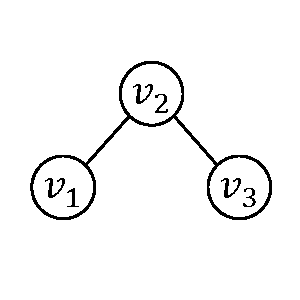
\includegraphics[width=0.9\linewidth]{is} 
\caption{Graph $G$}
\label{fig:is}
\end{subfigure}
\begin{subfigure}{0.66\textwidth}
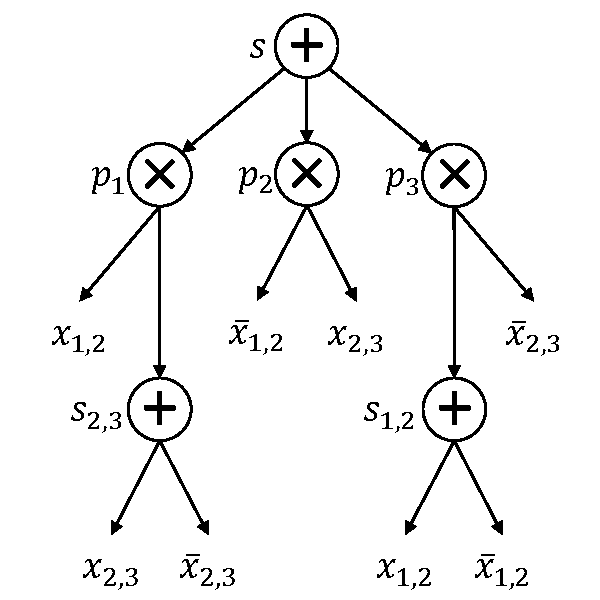
\includegraphics[width=0.9\linewidth]{auxspn}
\caption{Auxiliary SPN $S$}
\label{fig:auxspn}
\end{subfigure}

\caption{An instance of MAX-IS and the corresponding auxiliary SPN}
\label{fig:isauxspn}
\end{figure}

Figure \ref{fig:isauxspn} shows an example of the definition \ref{thm:auxspn}.

\begin{lemma}
Let graph $G(V, E)$ be an arbitrary instance of MAX-IS and let $S$ be the corresponding auxiliary SPN.
\begin{enumerate}
    \item Given any independent set of size $k$ in $G$, we can find an $x \in val(X)$ such that $S(x) \geq k$.
    \item Given any $x \in val(X)$ for which $S(x) = k$, we can find an  independent set of size $k$ in $G$.
\end{enumerate}
\end{lemma}
\begin{proof}
\textbf{Part 1:} Let $V'$ be the given independent set. $\forall (v_i, v_j) \in E$, let 
\[
X_{i, j} =
  \begin{cases}
    true, & \text{if $v_i \in V'$,}\\
    false, & \text{if $v_j \in V'$,}\\
    \text{arbitrary value}, & \text{otherwise.}
  \end{cases}    
\]
It is impossible that both $v_i, v_j \in V'$, since $(v_i, v_j) \in E$ and $V'$ is an independent set. Thus $\forall v_i \in V', p_i(x) = 1$ where $x$ is the corresponding assignment of $X$. Thus $S(x) \geq \left|V'\right| = k$.

\textbf{Part 2:} Let $x$ be the given assignment of $X$. Since $p_i(x)$ is either 0 or 1 and $\sum{p_i(x)}=k$, there are k product nodes $p_i(x) = 1$. We construct an independent set $V'=\{v_i \in V | p_i(x)=1\}$. So, $\left|V'\right| = k$. We show that $V'$ is an independent set. $\forall v_i, v_j \in V'$, if $(v_i, v_j) \in E$, there exists a variable $X_{i,j}$ with $x_{i,j}$ linked by $p_i$ and $\overline x_{i,j}$ linked by $p_j$. That means $p_i(x)$ and $p_j(x)$ cannot both be 1. This is conflict with $p_i(x)=1$ and $p_j(x)=1$. Therefore, $V'$ is an independent set with size k.
\end{proof}

\begin{corollary}
Let $G$ be an arbitrary instance of MAX-IS and let $S$ be the MPE instance of the corresponding auxiliary SPN. Let $k^\ast$ and $k'^\ast$ be the optimal solution of $G$ and $S$. Then, $k^\ast = k'^\ast$.
\end{corollary}

\begin{lemma}
If there is an approximation algorithm for MPE with a constant ratio $\rho$ in polynomial time, then there is an approximation algorithm for MAX-IS with the same constant ratio $\rho$ in polynomial time.
\end{lemma}

\begin{proof}
Let $G$ be an arbitrary instance of MAX-IS and let $S$ be the MPE instance of the corresponding auxiliary SPN. Let $k^\ast$ be the optimal solution of $S$. Suppose we can approximate $S$ with a bound $\rho=k/k^\ast$, i.e., we can find a solution $k=\rho \times k^\ast$ for $S$. Furthermore, we can find a solution $k' = k$ for $G$. The approximation ratio of $G$ is $\rho'=k'/k^\ast = k/k^\ast = \rho$. Finally, all the above works are in polynomial time.
\end{proof}

\begin{corollary}
If MPE is in $APX$, then MAX-IS is also in APX.
\end{corollary}

\begin{theorem}
MPE is not in $APX$ unless $P=NP$.
\end{theorem}
\begin{proof}
Suppose $P \neq NP$. Suppose MPE is in $APX$. Thus MAX-IS is in $APX$. This is conflict with the fact MAX-IS is not in $APX$ if $P \neq NP$.
\end{proof}
\end{document}
